% Changing book to article will make the footers match on each page,
% rather than alternate every other.
%
% Note that the article class does not have chapters.
\documentclass[letterpaper,10pt,twoside,twocolumn,openany]{book}

% Use babel or polyglossia to automatically redefine macros for terms
% Armor Class, Level, etc...
% Default output is in English; captions are located in lib/dndstring-captions.sty.
% If no captions exist for a language, English will be used.
%1. To load a language with babel:
%	\usepackage[<lang>]{babel}
%2. To load a language with polyglossia:
%	\usepackage{polyglossia}
%	\setdefaultlanguage{<lang>}
\usepackage[english]{babel}
%usepackage[italian]{babel}
% For further options (multilanguage documents, hypenations, language environments...)
% please refer to babel/polyglossia's documentation.

\usepackage[utf8]{inputenc}
\usepackage{hang}
\usepackage{lipsum}
\usepackage{listings}
\usepackage{dnd}
\usepackage{gensymb}

\lstset{%
  basicstyle=\ttfamily,
  language=[LaTeX]{TeX},
}

% Start document
\begin{document}

% Your content goes here

% Comment this out if you're using the article class.
\chapter{Rubik's Cube: Corners First Lösung}

\section{1) Ecken orientieren}
\begin{justify}
Im ersten Schritt werden alle 8 Ecken richtig orientiert, so dass sie mit den Mittelteilchen von allen Seiten überein stimmen.
\end{justify}

\subsection{Ecken der ersten Seite platzieren}
\begin{justify}
Dieser Schritt ist relativ einfach und erfolgt ohne Anleitung. Er ist abgeschlossen, sobald auf einer Würfelseite die Farben der 4 Ecken mit der Farbe des Mittelteilchens übereinstimmen - in der Abb. weiss markiert:
\end{justify}

\begin{figure}[!htb] 
  \centering
     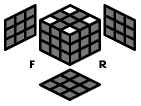
\includegraphics[width=0.20\textwidth]{img/white_corners.png}
\end{figure}
\subsection{Ecken der zweiten Seite platzieren}
\begin{justify}
Ist der vorangehende Schritt abgeschlossen, wird der Würfel so um 180\degree gedreht, dass die bearbeitete Seite nach unten zeigt. Dann werden die Ecken der nun nach oben zeigenden Seite, im Bild gelb markiert, gelöst:
\end{justify}

\begin{figure}[!htb] 
  \centering
     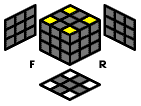
\includegraphics[width=0.20\textwidth]{img/yellow_corners.png}
\end{figure}
\begin{justify}
Um dies zu erreichen muss nun die anzuwendende Zugfolge, abhängig von der Lage der gelb markierten Ecken, ermittelt werden (F=front, R=right, U=upper, C=center, d.h. horizontale Zwischenebene; die Appostrophe kennzeichnen Drehungen im Gegenuhrzeigersinn bei senkrechtem Blick auf die jeweilige Ebene):
\end{justify}
\newpage
\subsubsection{Buchstabe T-Muster}
\begin{figure}[!htb] 
  \centering
     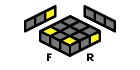
\includegraphics[width=0.20\textwidth]{img/t_pattern.png}
\end{figure}

\centering \textbf{Zugfolge:} R U R' U' F' U' F

\subsubsection{Buchstabe L-Muster}
\begin{figure}[!htb] 
  \centering
     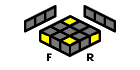
\includegraphics[width=0.20\textwidth]{img/l_pattern.png}
\end{figure}

\centering \textbf{Zugfolge:} F R' F' U' R' U R

\subsubsection{Sune \#1-Muster}
\begin{figure}[!htb] 
  \centering
     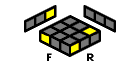
\includegraphics[width=0.20\textwidth]{img/sune_pattern_1.png}
\end{figure}

\centering \textbf{Zugfolge:} R U2 R' U' R U' R'


\subsubsection{Sune \#2-Muster}
\begin{figure}[!htb] 
  \centering
     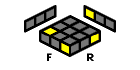
\includegraphics[width=0.20\textwidth]{img/sune_pattern_2.png}
\end{figure}
\centering \textbf{Zugfolge:} R U R' U R U2 R'

\subsubsection{Buchstabe $\pi$-Muster}
\begin{figure}[!htb] 
  \centering
     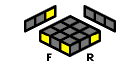
\includegraphics[width=0.20\textwidth]{img/pi_pattern.png}
\end{figure}

\centering \textbf{Zugfolge:} R U R2 F' R2 U R'

\newpage
\subsubsection{Buchstabe U-Muster}
\begin{figure}[!htb] 
  \centering
     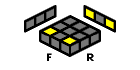
\includegraphics[width=0.20\textwidth]{img/u_pattern.png}
\end{figure}

\centering \textbf{Zugfolge:} R' F' U' F U R

\subsubsection{Buchstabe H-Muster}
\begin{figure}[!htb] 
  \centering
     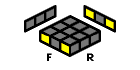
\includegraphics[width=0.20\textwidth]{img/h_pattern.png}
\end{figure}
\centering \textbf{Zugfolge:} R2 U2 R' U2 R2

\subsection{Alle Ecken richtig \newline orientieren}
\begin{justify}
In diesem Schritt werden alle 8 Ecken durch Anwenden einer einzigen Zugfolge richtig ausgerichtet. Um zu ermitteln, welche Zugfolge anzuwenden ist, müssen in der obersten und untersten Schicht die Würfelkanten gezählt werden, deren Ecken gleichfarbig sind. 
\end{justify}

\subsubsection{Kein Eckenpaar gleichfarbig}
\begin{figure}[!htb] 
  \centering
     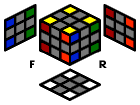
\includegraphics[width=0.20\textwidth]{img/orient-0-solved.png}
\end{figure}
\centering \textbf{Zugfolge:} F2 R2 F2
        
\subsubsection{Eckenpaar hinten unten\newline gleichfarbig}
\begin{figure}[!htb] 
  \centering
     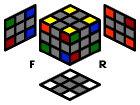
\includegraphics[width=0.20\textwidth]{img/orient-db-solved.png}
\end{figure}
\centering \textbf{Zugfolge:} R U' F U2 F' U R'

\subsubsection{Zwei Eckenpaare hinten\newline gleichfarbig}
\begin{figure}[!htb] 
  \centering
     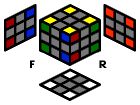
\includegraphics[width=0.20\textwidth]{img/orient-db-ub-solved.png}
\end{figure}
\centering \textbf{Zugfolge:} R2 U F2 U2 R2 U R2 

\subsubsection{Vier Eckenpaare unten\newline gleichfarbig}
\begin{figure}[!htb] 
  \centering
     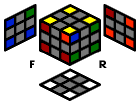
\includegraphics[width=0.20\textwidth]{img/orient-4d-solved.png}
\end{figure}
\centering \textbf{Zugfolge:} F2 U' R U' R' U F2 U R U R' 

\subsubsection{Fünf Eckenpaare unten und oben hinten gleichfarbig}
\begin{figure}[!htb] 
  \centering
     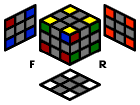
\includegraphics[width=0.20\textwidth]{img/orient-uf-not-solved.png}
\end{figure}
\centering \textbf{Zugfolge:} R U' R F2 R' U R F2 R2 
        
\section{2) Kanten der U/D-Ebenen positionieren}
\begin{justify}
Nachdem alle 8 Ecken korrekt orientiert sind, werden die Kanten - d.h. jene Teilchen mit zwei Stickern - der unteren und oberen Ebene korrekt platziert und orientiert. 
\end{justify}
\begin{figure}[!htb] 
  \centering
     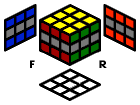
\includegraphics[width=0.20\textwidth]{img/set2solved.png}
\end{figure}

\subsection{Kanten platzieren und\newline orientieren}
\begin{justify}
Die Kantenteilchen werden jetzt Kante für Kante mit den nachfolgenden Zugfolgen platziert und orientiert. Man löst so zuerst die untere Ebene - bis auf eine Kante:
\begin{figure}[!htb] 
  \centering
     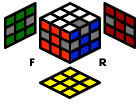
\includegraphics[width=0.20\textwidth]{img/single-gap-unsolved.png}
\end{figure}
\end{justify}

\subsubsection{Kante von hinten nach vorne unten}
\begin{figure}[!htb] 
  \centering
     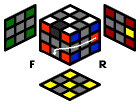
\includegraphics[width=0.20\textwidth]{img/hinten-rechts-vorne-unten.png}
\end{figure}
\centering \textbf{Zugfolge:} F' C F

\subsubsection{Kante von hinten nach vorne unten\newline gedreht}
\begin{figure}[!htb] 
  \centering
     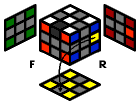
\includegraphics[width=0.20\textwidth]{img/hinten-rechts-vorne-unten-2.png}
\end{figure}
\centering \textbf{Zugfolge:} F C2 F'

\subsubsection{Kante von oben nach unten}
\begin{figure}[!htb] 
  \centering
     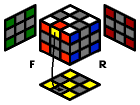
\includegraphics[width=0.20\textwidth]{img/oben-nach-unten.png}
\end{figure}
\centering \textbf{Zugfolge:} F C F'

\newpage
\subsubsection{Kante von oben nach unten\newline gedreht}
\begin{figure}[!htb] 
  \centering
     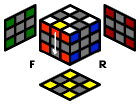
\includegraphics[width=0.20\textwidth]{img/oben-nach-unten2.png}
\end{figure}
\centering \textbf{Zugfolge:} F C' F2 C F

\subsubsection{Kante vorne unten kippen}
\begin{figure}[!htb] 
  \centering
     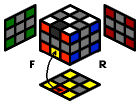
\includegraphics[width=0.20\textwidth]{img/oben-unten-nach-unten-twist.png}
\end{figure}
\centering{\textbf{Zugfolge:} F' C' F2 C2 F'}

\begin{justify}
Wurden drei beliebige Kanten in der unteren Ebene korrekt platziert und orientiert, wird die Untenseite nach oben gedreht und die vier Kantenteilchen der jetzt nach unten zeigenden Seite platziert und orientiert.

\indent Dabei ist zu beachten, dass die ungelöste Kante der oberen Seite immer gegenüber dem Kantenteilchen des zu lösenden Kantenteilchens der Unterseite positioniert wird. 
\end{justify}

\subsection{Letzte Kante lösen}
\begin{justify}
Jetzt muss noch die letzte Kante der Würfeloberseite gelöst werden. Je nach  Situation muss eine der folgenden 3 Zugfolgen eingesetzt werden:
\end{justify}
\subsubsection{Kante kippen}
\begin{figure}[!htb] 
  \centering
     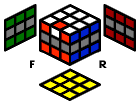
\includegraphics[width=0.20\textwidth]{img/swap_cant.png}
\end{figure}
\centering{\textbf{Zugfolge:} F C' F C' F C' F}
\newpage
\subsubsection{Kante von hinten rechts nach \newline vorne oben}
\begin{figure}[!htb] 
  \centering
     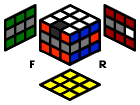
\includegraphics[width=0.20\textwidth]{img/stopf_easy.png}
\end{figure}
\centering{\textbf{Zugfolge:} F C' F' C F C F'}

\subsubsection{Kante von hinten rechts nach \newline vorne oben gedreht}
\begin{figure}[!htb] 
  \centering
     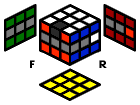
\includegraphics[width=0.20\textwidth]{img/stopf_hard.png}
\end{figure}
\centering{\textbf{Zugfolge:} F C' F2 C' F}

\subsection{Mittelelbene lösen}
\begin{justify}
Jetzt muss noch die verbleibende mittlere Ebene gelöst werden. Die Notation ändert sich hier leicht, F=front, U=upper, B=back, $\wedge$=mittlere Schicht nach oben, $\vee$=mittlere Schicht nach unten.
\end{justify}
\subsubsection{Kanten permutieren}
\begin{justify}
Diese Zugfolge ist dann zu wählen, wenn die einzig korrekte Kante der mittleren Schicht hinten unten liegt und die vorne oben liegende Kante nach vorne unten wandern soll:
\end{justify}
\begin{figure}[!htb] 
  \centering
     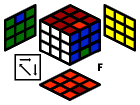
\includegraphics[width=0.20\textwidth]{img/middle-permutate.png}
\end{figure}
\centering{\textbf{Zugfolge:} $\wedge$ U2 $\vee$ U2}
\newpage
\subsubsection{Kanten horizontal tauschen}
\begin{justify}
Diese Zugfolge ist dann zu wählen, wenn die Kantenteilchen der Mittelschicht horizontal ausgetauscht werden sollen.  
\end{justify}
\begin{figure}[!htb] 
  \centering
     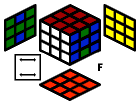
\includegraphics[width=0.20\textwidth]{img/middle-translate.png}
\end{figure}
\centering{\textbf{Zugfolge:} $\wedge\wedge$ U2 $\wedge\wedge$ U2}

\subsubsection{Kanten diagonal tauschen}
\begin{justify}
Diese Zugfolge ist dann zu wählen, wenn die Kantenteilchen der Mittelschicht diagonal ausgetauscht werden sollen.
\end{justify}
\begin{figure}[!htb] 
  \centering
     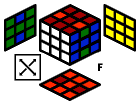
\includegraphics[width=0.20\textwidth]{img/middle-crossover.png}
\end{figure}
\centering{\textbf{Zugfolge:} $\wedge$ F2 B2 $\vee$ F2 B2}

\subsubsection{Obere Kanten der Mittelschicht kippen}
\begin{justify}
Diese Zugfolge ist dann zu wählen, wenn die Kantenteilchen der Mittelschicht diagonal ausgetauscht werden sollen.
\end{justify}
\begin{figure}[!htb] 
  \centering
     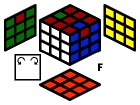
\includegraphics[width=0.20\textwidth]{img/middle-topswap.png}
\end{figure}
\centering{\textbf{Zugfolge:} $\wedge$ U $\wedge$ U $\wedge$ U2 $\vee$ U $\vee$ U $\vee$ U2} 

\begin{justify}
Liegen 2 diagonal gegenüber liegende gekippte Kantenteilchen vor, so kann der Würfel durch eine Drehung der Frontseite oder Rückseite auf dasselbe Problem zurückgeführt werden, so dass dan wieder die Zugfolge zum 
\end{justify}

\subsubsection{Alle Kanten der Mittelschicht \newline kippen}
\begin{justify}
Relativ selten kommt es vor, dass alle 4 Eckpunkte der Mittelschicht gekippt werden müssen. In diesen Fällen ist 
\end{justify}
\begin{figure}[!htb] 
  \centering
     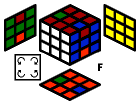
\includegraphics[width=0.20\textwidth]{img/middle-allswap.png}
\end{figure}
\centering{\textbf{Zugfolge:} $\wedge$ U $\wedge$ U $\wedge$ U2 $\vee$ U $\vee$ U $\vee$ U2} 


% End document
\end{document}
